\documentclass{standalone}
\usepackage{tikz}
\usepackage{xcolor}
\usetikzlibrary{patterns, positioning}
\usetikzlibrary{shapes.misc}
\usepackage[outline]{contour}
\contourlength{1.5pt} 


\begin{document}
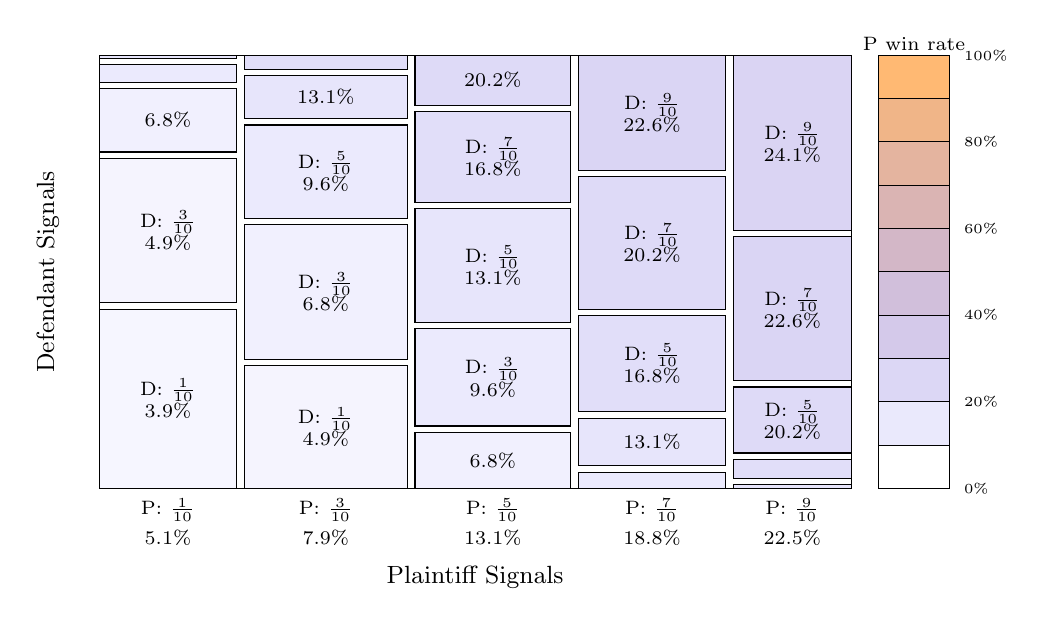
\begin{tikzpicture}
\newcommand{\DFractionOffset}{0.4}
\newcommand{\AxisLabelYAdjust}{-0.235}
\draw[draw=black] (0.6,2) rectangle (10.15,7.5);
\draw[fill=blue!96!orange!4!white!87!white, draw=black] (0.6,2) rectangle (2.3479,4.2767);
\draw (1.4739318529603298, 3.138353264977417) node[font=\scriptsize, text=black, align=center] {D: $\frac{1}{10}$\\ 3.9\%};
\draw[fill=blue!95!orange!5!white!86!white, draw=black] (0.6,4.3567) rectangle (2.3479,6.1926);
\draw (1.4739318529603298, 5.2746395503078265) node[font=\scriptsize, text=black, align=center] {D: $\frac{3}{10}$\\ 4.9\%};
\draw[fill=blue!93!orange!7!white!86!white, draw=black] (0.6,6.2726) rectangle (2.3479,7.079);
\draw (1.4739318529603298, 6.675806688297891) node[font=\scriptsize, text=black, align=center] {6.8\%};
\draw[fill=blue!90!orange!10!white!85!white, draw=black] (0.6,7.159) rectangle (2.3479,7.3795);
\draw[fill=blue!87!orange!13!white!84!white, draw=black] (0.6,7.4595) rectangle (2.3479,7.5);
\draw (1.4739318529603298, 1.6) node[anchor=north, font=\scriptsize, text=black] {5.1\%};
\draw (1.4739318529603298, {1.6 + \DFractionOffset}) node[anchor=north, font=\scriptsize, text=black] {P: $\frac{1}{10}$};
\draw[fill=blue!95!orange!5!white!86!white, draw=black] (2.4479,2) rectangle (4.5113,3.5551);
\draw (3.4795799975611055, 2.7775499057934168) node[font=\scriptsize, text=black, align=center] {D: $\frac{1}{10}$\\ 4.9\%};
\draw[fill=blue!93!orange!7!white!86!white, draw=black] (2.4479,3.6351) rectangle (4.5113,5.3527);
\draw (3.4795799975611055, 4.493901344809022) node[font=\scriptsize, text=black, align=center] {D: $\frac{3}{10}$\\ 6.8\%};
\draw[fill=blue!90!orange!10!white!85!white, draw=black] (2.4479,5.4327) rectangle (4.5113,6.6156);
\draw (3.4795799975611055, 6.024162911239146) node[font=\scriptsize, text=black, align=center] {D: $\frac{5}{10}$\\ 9.6\%};
\draw[fill=blue!87!orange!13!white!84!white, draw=black] (2.4479,6.6956) rectangle (4.5113,7.2449);
\draw (3.4795799975611055, 6.970237664553861) node[font=\scriptsize, text=black, align=center] {13.1\%};
\draw[fill=blue!83!orange!17!white!82!white, draw=black] (2.4479,7.3249) rectangle (4.5113,7.5);
\draw (3.4795799975611055, 1.6) node[anchor=north, font=\scriptsize, text=black] {7.9\%};
\draw (3.4795799975611055, {1.6 + \DFractionOffset}) node[anchor=north, font=\scriptsize, text=black] {P: $\frac{3}{10}$};
\draw[fill=blue!93!orange!7!white!86!white, draw=black] (4.6113,2) rectangle (6.5882,2.713);
\draw (5.599727989038177, 2.356523510589186) node[font=\scriptsize, text=black, align=center] {6.8\%};
\draw[fill=blue!90!orange!10!white!85!white, draw=black] (4.6113,2.793) rectangle (6.5882,4.0278);
\draw (5.599727989038177, 3.4104077879523294) node[font=\scriptsize, text=black, align=center] {D: $\frac{3}{10}$\\ 9.6\%};
\draw[fill=blue!87!orange!13!white!84!white, draw=black] (4.6113,4.1078) rectangle (6.5882,5.5495);
\draw (5.599727989038177, 4.828647074880229) node[font=\scriptsize, text=black, align=center] {D: $\frac{5}{10}$\\ 13.1\%};
\draw[fill=blue!83!orange!17!white!82!white, draw=black] (4.6113,5.6295) rectangle (6.5882,6.7876);
\draw (5.599727989038177, 6.208570133361866) node[font=\scriptsize, text=black, align=center] {D: $\frac{7}{10}$\\ 16.8\%};
\draw[fill=blue!80!orange!20!white!81!white, draw=black] (4.6113,6.8676) rectangle (6.5882,7.5);
\draw (5.599727989038177, 7.18380733584478) node[font=\scriptsize, text=black, align=center] {20.2\%};
\draw (5.599727989038177, 1.6) node[anchor=north, font=\scriptsize, text=black] {13.1\%};
\draw (5.599727989038177, {1.6 + \DFractionOffset}) node[anchor=north, font=\scriptsize, text=black] {P: $\frac{5}{10}$};
\draw[fill=blue!90!orange!10!white!85!white, draw=black] (6.6882,2) rectangle (8.558,2.2061);
\draw[fill=blue!87!orange!13!white!84!white, draw=black] (6.6882,2.2861) rectangle (8.558,2.8922);
\draw (7.623063100641959, 2.589122351312139) node[font=\scriptsize, text=black, align=center] {13.1\%};
\draw[fill=blue!83!orange!17!white!82!white, draw=black] (6.6882,2.9722) rectangle (8.558,4.1966);
\draw (7.623063100641959, 3.584372469333866) node[font=\scriptsize, text=black, align=center] {D: $\frac{5}{10}$\\ 16.8\%};
\draw[fill=blue!80!orange!20!white!81!white, draw=black] (6.6882,4.2766) rectangle (8.558,5.9576);
\draw (7.623063100641959, 5.1171044614162415) node[font=\scriptsize, text=black, align=center] {D: $\frac{7}{10}$\\ 20.2\%};
\draw[fill=blue!77!orange!23!white!81!white, draw=black] (6.6882,6.0376) rectangle (8.558,7.5);
\draw (7.623063100641959, 6.768819238288827) node[font=\scriptsize, text=black, align=center] {D: $\frac{9}{10}$\\ 22.6\%};
\draw (7.623063100641959, 1.6) node[anchor=north, font=\scriptsize, text=black] {18.8\%};
\draw (7.623063100641959, {1.6 + \DFractionOffset}) node[anchor=north, font=\scriptsize, text=black] {P: $\frac{7}{10}$};
\draw[fill=blue!87!orange!13!white!84!white, draw=black] (8.658,2) rectangle (10.15,2.0475);
\draw[fill=blue!83!orange!17!white!82!white, draw=black] (8.658,2.1275) rectangle (10.15,2.3697);
\draw[fill=blue!80!orange!20!white!81!white, draw=black] (8.658,2.4497) rectangle (10.15,3.2876);
\draw (9.403983256204555, 2.868619899643248) node[font=\scriptsize, text=black, align=center] {D: $\frac{5}{10}$\\ 20.2\%};
\draw[fill=blue!77!orange!23!white!81!white, draw=black] (8.658,3.3676) rectangle (10.15,5.2002);
\draw (9.403983256204555, 4.283869074053512) node[font=\scriptsize, text=black, align=center] {D: $\frac{7}{10}$\\ 22.6\%};
\draw[fill=blue!76!orange!24!white!80!white, draw=black] (8.658,5.2802) rectangle (10.15,7.5);
\draw (9.403983256204555, 6.39009006398214) node[font=\scriptsize, text=black, align=center] {D: $\frac{9}{10}$\\ 24.1\%};
\draw (9.403983256204555, 1.6) node[anchor=north, font=\scriptsize, text=black] {22.5\%};
\draw (9.403983256204555, {1.6 + \DFractionOffset}) node[anchor=north, font=\scriptsize, text=black] {P: $\frac{9}{10}$};
\node[font=\small, text=black] at (5.375, {1.1 + \AxisLabelYAdjust}) {Plaintiff Signals};
\node[font=\small, text=black, rotate=90] at (-0.050000000000000044, 4.75) {Defendant Signals};
\draw[draw=black] (10.5,2) rectangle (11.4,7.5);
\draw (10.95, 7.65) node[font=\scriptsize, text=black] {P win rate};
\draw[fill=blue!100!orange!0!white!88!white, draw=black] (10.5,2) rectangle (11.4,2.55);
\draw[fill=blue!89!orange!11!white!84!white, draw=black] (10.5,2.55) rectangle (11.4,3.1);
\draw[fill=blue!78!orange!22!white!81!white, draw=black] (10.5,3.1) rectangle (11.4,3.65);
\draw[fill=blue!67!orange!33!white!77!white, draw=black] (10.5,3.65) rectangle (11.4,4.2);
\draw[fill=blue!56!orange!44!white!73!white, draw=black] (10.5,4.2) rectangle (11.4,4.75);
\draw[fill=blue!44!orange!56!white!70!white, draw=black] (10.5,4.75) rectangle (11.4,5.3);
\draw[fill=blue!33!orange!67!white!66!white, draw=black] (10.5,5.3) rectangle (11.4,5.85);
\draw[fill=blue!22!orange!78!white!62!white, draw=black] (10.5,5.85) rectangle (11.4,6.4);
\draw[fill=blue!11!orange!89!white!59!white, draw=black] (10.5,6.4) rectangle (11.4,6.95);
\draw[fill=blue!0!orange!100!white!55!white, draw=black] (10.5,6.95) rectangle (11.4,7.5);
\draw (11.46, 2) node[anchor=west, font=\tiny, text=black] {0\%};
\draw (11.46, 3.1) node[anchor=west, font=\tiny, text=black] {20\%};
\draw (11.46, 4.2) node[anchor=west, font=\tiny, text=black] {40\%};
\draw (11.46, 5.3) node[anchor=west, font=\tiny, text=black] {60\%};
\draw (11.46, 6.4) node[anchor=west, font=\tiny, text=black] {80\%};
\draw (11.46, 7.5) node[anchor=west, font=\tiny, text=black] {100\%};


\end{tikzpicture}
\end{document}